\section{Physics Requirements}

\subsection{Performance Criteria}

The design parameters of the PCAL were established using full GEANT simulations of the PCAL-EC system
(together referred to as the ECAL). These studies are described in detail in Ref.~\cite{2007001} and
summarized below. The mechanical design depends on the number of scintillator-lead layers, on the angular
coverage of the PCAL, and on the degree of readout segmentation. These parameters were determined by
the physics requirements for the detection and identification of high energy electrons, photons, and $\pi^{0}$
mesons via $2\gamma$\ decay.

\begin{figure}[hbt]
\centering
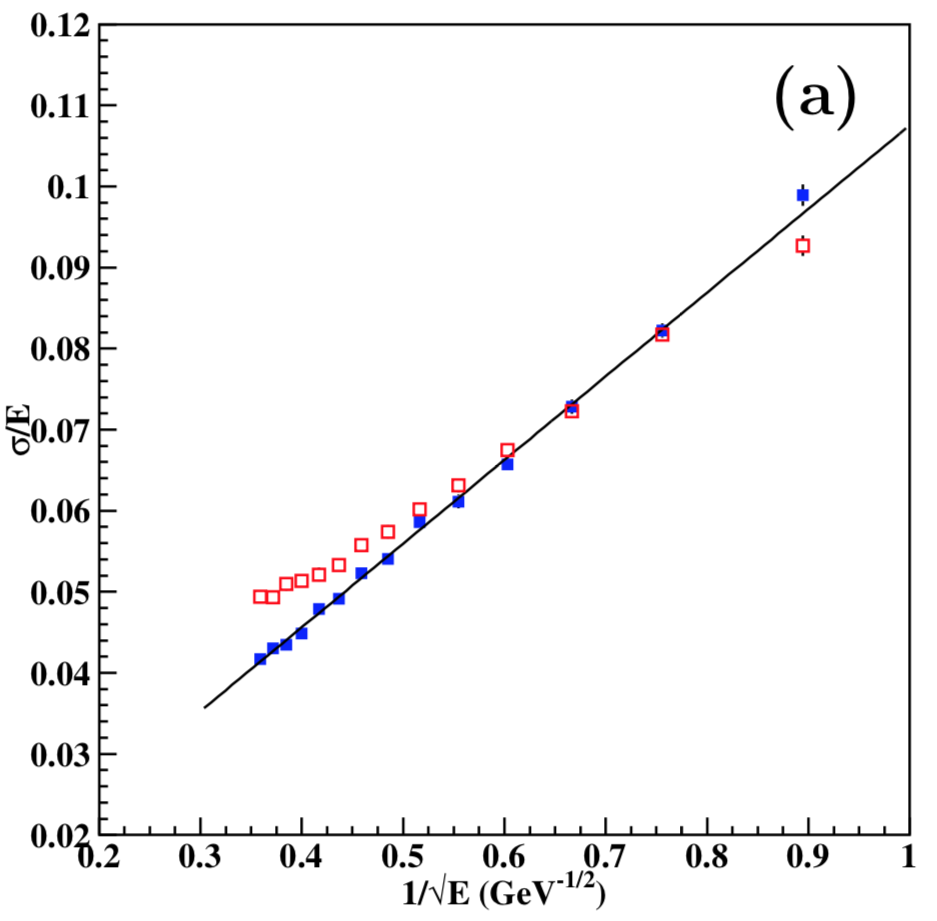
\includegraphics[width=0.85\columnwidth,keepaspectratio]{img/S2_1_a.png}
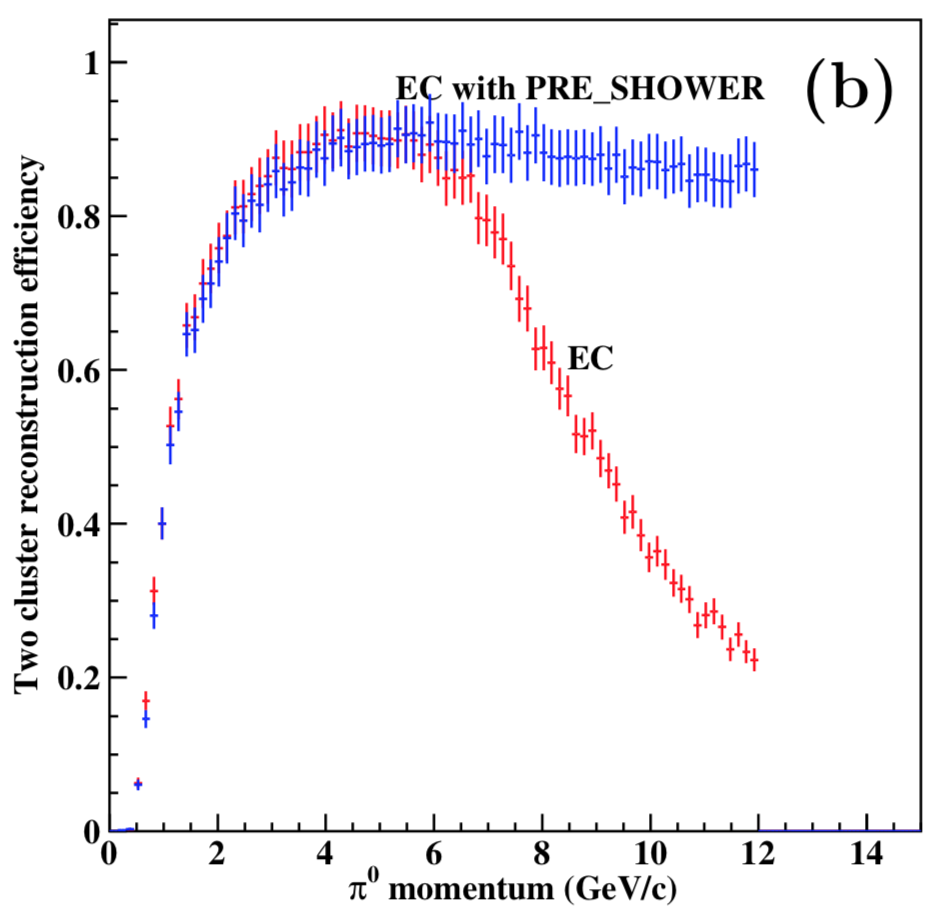
\includegraphics[width=0.85\columnwidth,keepaspectratio]{img/S2_1_b.png}
\caption[Simulated performance]{Comparison of simulated performance of the combined PCAL+EC calorimeter
  (blue points) and EC only (red points) at CLAS12 energies. a) Energy resolution as a function of inverse square
  root of energy. b) Reconstruction efficiency of two clusters from $\pi^{0}$ decay photons as a function of pion
  momentum.}
\label{fig:S2_1}
\end{figure}

Initial simulations were carried out with 15 layers of lead and scintillator (similar to the inner part of the EC),
using 3.5~cm wide segmentation for the scintillator layers, corresponding to about 108 readout channels in each
stereo view. For comparison the EC uses 10 cm wide strips. Events were generated using a uniform distribution
of $\pi^{0}\rightarrow 2\gamma$ decays at the target with momenta up to 12~GeV. Showers were identified
using the standard cluster reconstruction algorithm of the EC, but applied to both PCAL and EC. As shown in
Fig.~\ref{fig:S2_1}, the combined PCAL and EC system retains good energy resolution,
$\sigma/E \approx 0.1 \times E^{-1/2}$, with constant efficiency for two cluster reconstruction up to the highest
momenta.

Additional simulations were performed using variable segmentation of the scintillator layers. Keeping constant
the total number of readout channels per sector, it was found that the maximum efficiency can be obtained if half
of each stereo layer is equipped with 4.5~cm strips and half with 9.0~cm strips (double strip readout). The triangular
stereo layers overlap such that there is always a region with 4.5~cm strips in one of the stereo layers, as shown in
Fig.~\ref{fig:S2_2}. There is only a small loss of two-cluster efficiency at the highest momenta for this geometry
compared with 4.5~cm strips in all stereo layers. It should be noted that at forward angles (short U-strips) where
most of the high energy $\pi^{0}$ are produced, all three stereo readout views have the high density readout
segmentation needed to resolve the small $2\gamma$ opening angles of $<3^{\circ}$.

\begin{figure}[hbt]
\centering
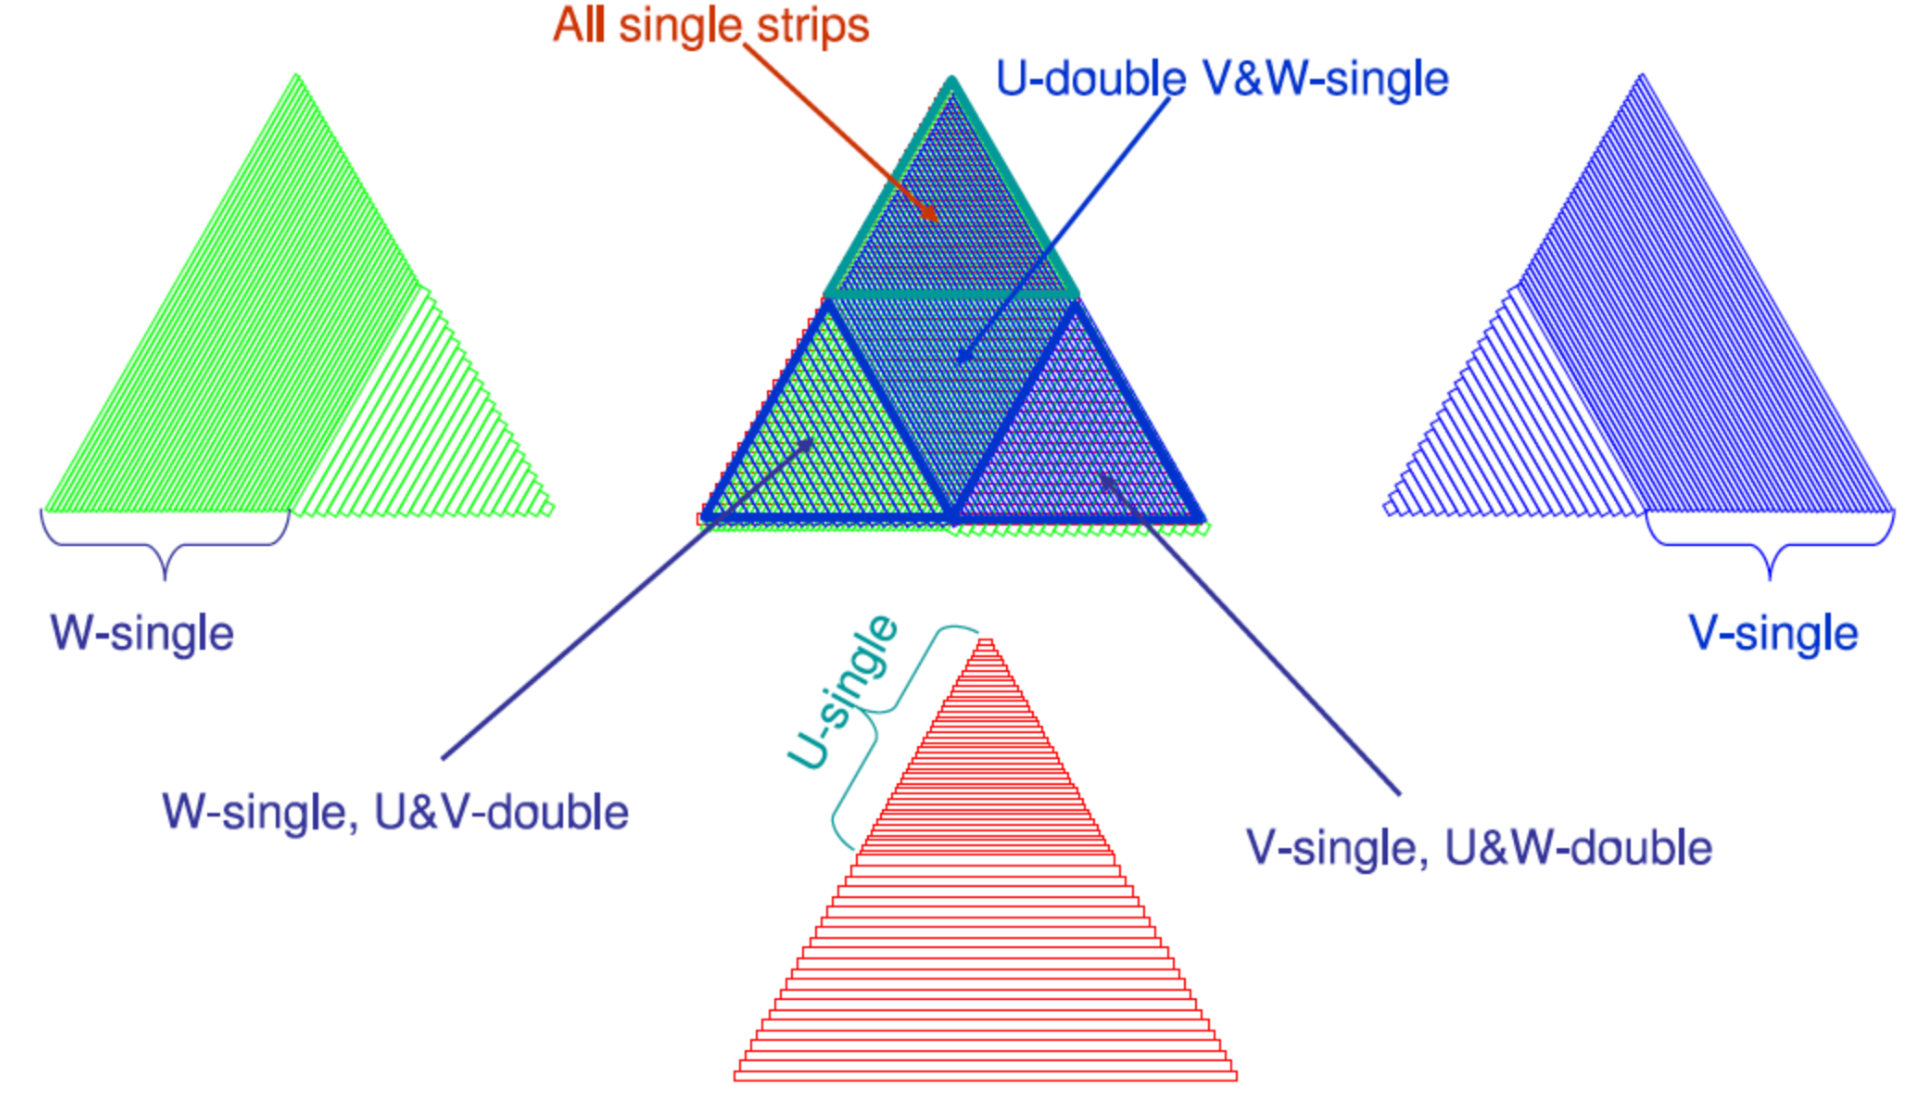
\includegraphics[width=0.95\columnwidth,keepaspectratio]{img/S2_2.png}
\caption{Segmentation pattern for different PCAL stereo readout planes (U, V, and W). There is always a region
  with single strip width (4.5~cm) segmentation in one of the stereo layers. The U PMTs are read out from the
  left side of the triangle, as seen in this view from the target, while the V and W PMTs are read out from the base.}
\label{fig:S2_2}
\end{figure}



